\documentclass[8pt,a4paper,compress]{beamer}

\usepackage{/home/siyer/lib/slides}

\title{Data Abstraction}
\date{}

\begin{document}
\begin{frame}
\vfill
\titlepage
\end{frame}

\begin{frame}
\frametitle{Outline}
\tableofcontents
\end{frame}

\section{Using Abstract Data Types}
\begin{frame}[fragile]
\begin{itemize}
\item an abstract data type (ADT) is a data type whose representation is hidden from the client

\item we use an API to specify the behavior of an abstract data type

\item \lstinline{Counter} data type
\begin{lstlisting}[language={},mathescape]
public class Counter implements Comparable<Counter> 

    Counter(String id) // create a counter named $id$
    void increment()   // increment the counter by one
    int tally()        // number of increments since creation
    String toString()  // string representation
    ...
\end{lstlisting}

\item similarities with a library of static methods
\begin{itemize}
\item both are implemented as a Java class
\item instance methods may take zero or more arguments of a specified type, separated by commas and enclosed in parentheses
\item they may provide a return value of a specified type or no return value (signified by \lstinline{void})
\end{itemize}

\item differences from a library of static methods
\begin{itemize}
\item some entries (called constructors) have the same name as the class and lack a return type
\item instance methods lack the \lstinline{static} modifier, and their purpose is to operate on data type values
\item some instance methods (called inherited methods) are present so as to follow Java conventions
\end{itemize}
\end{itemize}
\end{frame}

\begin{frame}[fragile]
\begin{itemize}
\item every Java data type inherits from \lstinline{java.lang.Object}, the \lstinline{toString()}, \lstinline{equals()}, and \lstinline{hashCode()} methods

\item an API for a data type allows us to write client code without knowing details of the implementation

\item an object is an entity that can take on a data-type value

\item objects are characterized by: state, which is a value from its data type; identity (place in memory), which distinguishes one object from another; and behavior, which is the effect of data-type operations

\item to create (or instantiate) an object, we invoke a constructor by using the keyword \lstinline{new} followed by the class name, followed by \lstinline{()} (or a list of argument values enclosed in parentheses, if the constructor takes arguments)

\begin{lstlisting}[language=Java]
Counter heads = new Counter("heads");
Counter tails = new Counter("tails");
\end{lstlisting}

\begin{center}
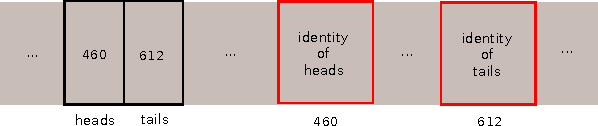
\includegraphics[scale=0.8]{./figures/obj_rep.pdf}
\end{center}
\end{itemize}
\end{frame}

\begin{frame}[fragile]
\begin{itemize}
\item the purpose of an instance method is to operate on data-type values

\item an instance method is invoked by writing a variable name that refers to an object, followed by a period, followed by an instance method name, followed by 0 or more arguments, enclosed in parentheses and separated by commas 

\item simulating $T$ coin flips
\begin{lstlisting}[language=Java]
public class Flips {
    public static void main(String[] args) {
        int T = Integer.parseInt(args[0]);
        Counter heads = new Counter("heads");
        Counter tails = new Counter("tails");
        for (int t = 0; t < T; t++) {
            if (StdRandom.bernoulli(0.5)) {
                heads.increment();
            }
            else {
                tails.increment();
            }
        }
        StdOut.println(heads);
        StdOut.println(tails);
        int delta = heads.tally() - tails.tally();
        StdOut.println("delta: " + Math.abs(delta));
    }
}
\end{lstlisting}

\begin{lstlisting}[language={}]
$ java Flips 1000000
499422 heads
500578 tails
delta: 1156
\end{lstlisting}
\end{itemize}
\end{frame}

\begin{frame}[fragile]
\begin{itemize}
\item an assignment statement with a reference type creates a copy (an alias) of the reference, not a new object

\item you can pass objects as arguments to methods and you can also use an object as a return value from a method

\item simulating $T$ coin flips and finding out who (heads or tails) is the winner
\begin{lstlisting}[language=Java]
public class FlipsMax {
    public static Counter max(Counter x, Counter y) {
        return x.tally() > y.tally() ? x : y;
    }

    public static void main(String[] args) {
        int T = Integer.parseInt(args[0]);
        Counter heads = new Counter("heads");
        Counter tails = new Counter("tails");
        for (int t = 0; t < T; t++) {
            if (StdRandom.bernoulli(0.5)) { heads.increment(); }
            else { tails.increment(); }
        }
        if (heads.tally() == tails.tally()) {
            StdOut.println("Tie");
        }
        else {
            StdOut.println(max(heads, tails) + " wins");
        }
    }
}
\end{lstlisting}

\begin{lstlisting}[language={}]
$ java FlipsMax 1000000
501181 heads wins
\end{lstlisting}
\end{itemize}
\end{frame}

\begin{frame}[fragile]
\begin{itemize}
\item in Java, every value of any nonprimitive type is an object, and in particular, arrays are objects 

\item array entries can be of any type, including reference types, ie, they can be objects

\item simulating $T$ rolls of a die
\begin{lstlisting}[language=Java]
public class Rolls {
    public static void main(String[] args) {
        int T = Integer.parseInt(args[0]);
        int SIDES = 6;
        Counter[] rolls = new Counter[SIDES + 1];
        for (int i = 1; i <= SIDES; i++) {
            rolls[i] = new Counter(i + "'s");
        }
        for (int t = 0; t < T; t++) {
            int result = StdRandom.uniform(1, SIDES + 1);
            rolls[result].increment();
        }
        for (int i = 1; i <= SIDES; i++) {
            StdOut.println(rolls[i]);
        }
    }
}
\end{lstlisting}

\begin{lstlisting}[language={}]
$ java Rolls 1000000
166674 1's
166337 2's
166566 3's
166926 4's
166822 5's
166675 6's
\end{lstlisting}
\end{itemize}
\end{frame}

\section{Examples of Abstract Data Types}
\begin{frame}[fragile]
\begin{itemize}
\item standard Java system types in \lstinline{java.lang}
\begin{lstlisting}[language={},mathescape]
Integer       // int wrapper
Double        // double wrapper
String        // indexed chars
StringBuilder // builder for strings
\end{lstlisting}

\item other Java Types
\begin{lstlisting}[language={},mathescape]
java.awt.Color // colors
java.awt.Font  // fonts
java.net.URL   // URLs
java.io.File   // files
\end{lstlisting}

\item standard IO types from the text
\begin{lstlisting}[language={},mathescape]
In   // input stream
Out  // output stream
Draw // drawing
\end{lstlisting}

\item data-oriented types for client examples
\begin{lstlisting}[language={},mathescape]
Point2D     // point in the plane
Interval1D  // 1D interval
Interval2D  // 2D interval
Date        // date
Transaction // transaction
\end{lstlisting}

\item types for analysis of algorithms
\begin{lstlisting}[language={},mathescape]
Counter           // counter
Accumulator       // accumulator
VisualAccumulator // visual version
Stopwatch         // stopwatch
\end{lstlisting}
\end{itemize}
\end{frame}

\begin{frame}[fragile]
\begin{itemize}
\item collection types
\begin{lstlisting}[language={},mathescape]
Stack                  // pushdown stack
Queue                  // FIFO queue
Bag                    // bag
MinPQ, MaxPQ           // priority queue
IndexMinPQ, IndexMaxPQ // priority queue (indexed)
ST                     // symbol table
SET                    // set
StringST               // symbol table (string keys)
\end{lstlisting}

\item data-oriented graph types
\begin{lstlisting}[language={},mathescape]
Graph               // graph
Digraph             // directed graph
Edge                // edge (weighted)
EdgeWeightedGraph   // graph (weighted)
DirectedEdge        // edge (directed, weighted)
EdgeWeightedDigraph // graph (directed, weighted)
\end{lstlisting}

\item operations-oriented graph types
\begin{lstlisting}[language={},mathescape]
UF                // dynamic connectivity
DepthFirstPaths   // DFS path searcher
CC                // connected components
BreadhFirstPaths  // BFS path searcher
DirectedDFS       // DFS digraph path search
DirectedBFS       // BFS digraph path search
TransitiveClosure // all paths
Topological       // topological order
DepthFirstOrder   // DFS order
DirectedCycle     // cycle search
SCC               // strong components
MST               // minimum spanning tree
SP                // shortest paths
\end{lstlisting}
\end{itemize}
\end{frame}

\begin{frame}[fragile]
\begin{itemize}
\item \lstinline{Point2D}
\begin{lstlisting}[language={},mathescape]
public class Point2D

    Point2D(double x, double y) // create a point
    double x()                  // $x$ coordinate
    double y()                  // $y$ coordinate
    double r()                  // radius (polar coordinates)
    double theta()              // angle (polar coordinates)
    double distTo(Point2D that) // distance from the point to that
    void draw()                 // draw the point on StdDraw
\end{lstlisting}

\item \lstinline{Interval1D}
\begin{lstlisting}[language={},mathescape]
public class Interval1D

    Interval1D(double lo, double hi)    // create an interval
    double length()                     // length of the interval
    boolean contains(double x)          // does the interval contain $x$?
    boolean intersects(Interval1D that) // does the interval intersect that?
    void draw()                         // draw the interval on StdDraw          
\end{lstlisting}

\item \lstinline{Interval2D}
\begin{lstlisting}[language={},mathescape]
public class Interval2D
          
    Interval2D(Interval1D x, Interval1D y) // create a 2D interval
    double area()                          // area of the 2D interval 
    boolean contains(Point2D p)            // does the interval contain p?
    boolean intersects(Interval2D that) // does the interval intersect that?
    void draw()                         // draw the interval on StdDraw
\end{lstlisting}
\end{itemize}
\end{frame}

\begin{frame}[fragile]
\begin{itemize}
\item \lstinline{Interval2D} test client
\begin{lstlisting}[language=Java]
public class Interval2D {
    ...
    public static void main(String[] args) {
        double xlo = Double.parseDouble(args[0]);
        double xhi = Double.parseDouble(args[1]);
        double ylo = Double.parseDouble(args[2]);
        double yhi = Double.parseDouble(args[3]);
        int T = Integer.parseInt(args[4]);
        Interval1D xinterval = new Interval1D(xlo, xhi);
        Interval1D yinterval = new Interval1D(ylo, yhi);
        Interval2D box = new Interval2D(xinterval, yinterval);
        box.draw();
        Counter counter = new Counter("hits");
        for (int t = 0; t < T; t++) {
            double x = StdRandom.uniform(0.0, 1.0);
            double y = StdRandom.uniform(0.0, 1.0);
            Point2D p = new Point2D(x, y);
            if (box.contains(p)) { counter.increment(); }
            else { p.draw(); }
        }
        StdOut.println(counter);
        StdOut.printf("box area = %.2f\n", box.area());
    }
}
\end{lstlisting}

\begin{minipage}{160pt}
\begin{lstlisting}[language={}]
$ java Interval2D 0.2 0.5 0.5 0.6 100000
3092 hits
box area = 0.03
\end{lstlisting}
\end{minipage}%
\begin{minipage}{120pt}
\hfill 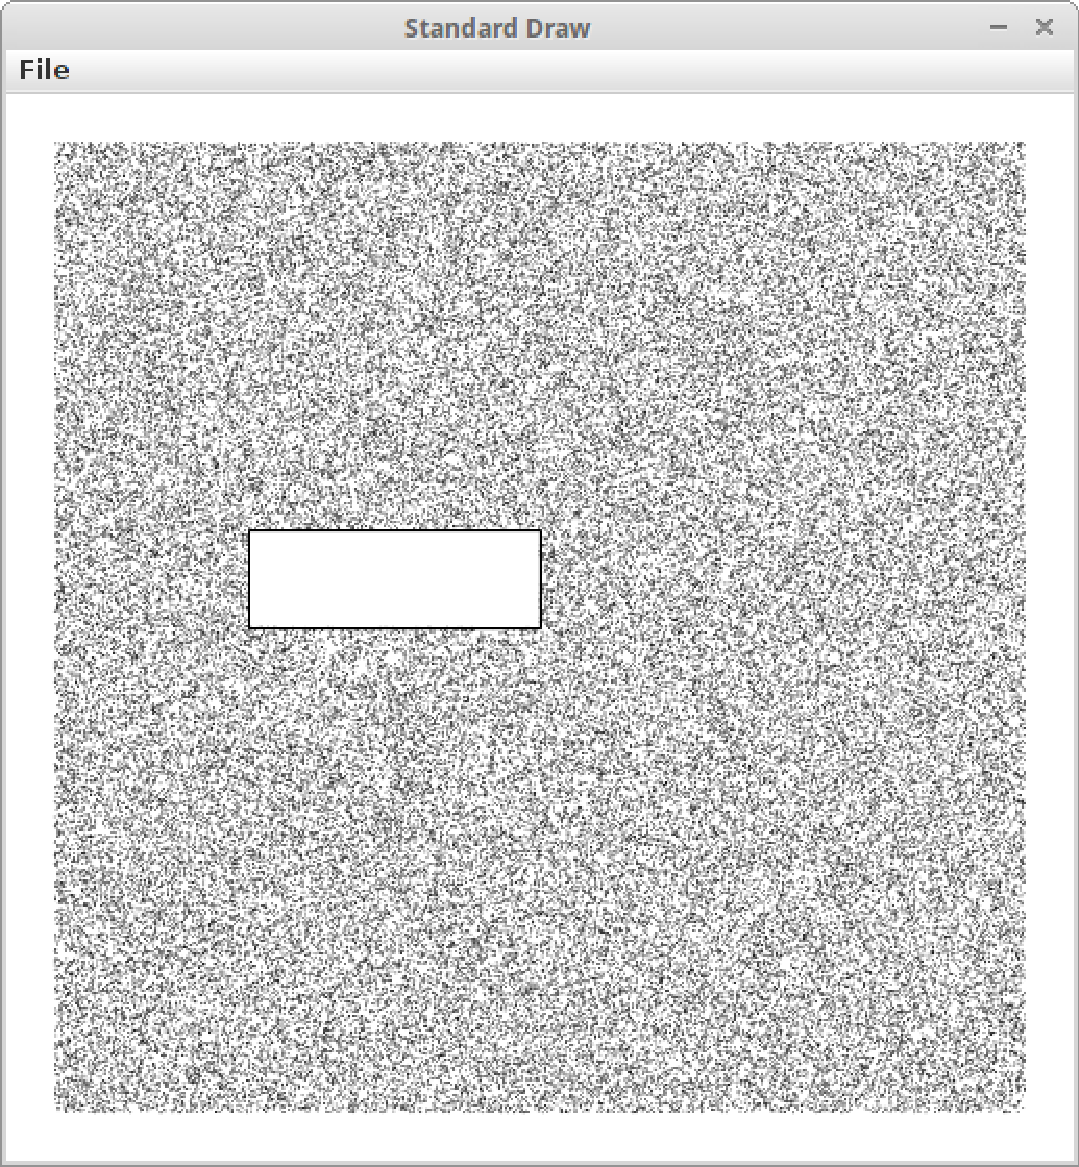
\includegraphics[scale=0.1]{./figures/interval2D.pdf}
\end{minipage}
\end{itemize}
\end{frame}

\begin{frame}[fragile]
\begin{itemize}
\item \lstinline{Date}
\begin{lstlisting}[language={},mathescape]
public class Date implements Comparable<Date>

    Date(int month, int day, int year) // create a date
    Date(String date)                  // create a date (parse constructor)
    int month()                        // month
    int day()                          // day
    int year()                         // year
    String toString()                  // string representation
    boolean equals(Object that)        // is the date same as that?
    int compareTo(Date that)           // compare the date to that
    int hashCode()                     // hash code
\end{lstlisting}

\item \lstinline{Transaction}
\begin{lstlisting}[language={},mathescape]
public class Transaction implements Comparable<Transaction>

    Transaction(String who, Date when, double amount) // create a 
                                                      // transaction
    Transaction(String transaction) // create a transaction 
                                    // (parse constructor)
    String who()                    // customer name
    Date when()                     // date
    double amount()                 // amount
    String toString()               // string representation
    boolean equals(Object that)     // is the transaction same as that?
    int compareTo(Transaction that) // compare the transaction to that
    int hashCode()                  // hash code
\end{lstlisting}
\end{itemize}
\end{frame}

\begin{frame}[fragile]
\begin{itemize}
\item \lstinline{String}

\begin{lstlisting}[language={},mathescape]
public class String implements Comparable<String>

    String()                     // create an empty string
    int length()                 // length of the string
    int charAt(int i)            // $i$th character
    int indexOf(String p)        // first occurrence of $p$ or -1
    int indexOf(String p, int i) // first occurrence of $p$ after $i$ or -1
    String concat(String t)        // the string with $t$ appended
    String substring(int i, int j) // substring of the string $[i, j)$
    String[] split(String delim)   // strings between occurrences of delim
    int compareTo(String t)        // string comparison
    boolean equals(String t)       // is the string's value the same as $t$'s?
    int hashCode()                 // hash code
    ...
\end{lstlisting}

\item \lstinline{In}
\begin{lstlisting}[language={},mathescape]
public class In

    In()                // create an input stream from standard input
    In(String name)     // create an input stream from a file or website
    int[] readInts()       // read int values
    double[] readDoubles() // read double values
    ...
\end{lstlisting}

\item \lstinline{Out}
\begin{lstlisting}[language={},mathescape]
public class Out

    Out()                  // create an output stream to standard output
    Out(String name)       // create an output stream to a file
    void write(int[] a)    // write int values
    void write(double[] a) // write double values
    ...
\end{lstlisting}
\end{itemize}
\end{frame}

\begin{frame}[fragile]
\begin{itemize}
\item \lstinline{In}/\lstinline{Out} client
\begin{lstlisting}[language=Java]
public class Cat { 
   public static void main(String[] args) { 
        Out out = new Out(args[args.length - 1]);
        for (int i = 0; i < args.length - 1; i++) {
            In in = new In(args[i]);
            String s = in.readAll();
            out.println(s);
            in.close();
        }
        out.close();
    }
}
\end{lstlisting}

\begin{lstlisting}[language={}]
$ more A.txt
To be, or not to be, 
$ more B.txt
that is the question.
$ java Cat A.txt B.txt C.txt
$ more C.txt
To be, or not to be, that is the question.
\end{lstlisting}

\item \lstinline{Draw}
\begin{lstlisting}[language={},mathescape]
public class Draw

    Draw()
    void line(double x0, double y0, double x1, double y1)
    void point(double x, double y)
    void text(double x, double y, String s)
    ...
\end{lstlisting}
\end{itemize}
\end{frame}

\section{Implementing an Abstract Data Type}
\begin{frame}[fragile]
\begin{itemize}
\item we implement ADTs with a Java class, putting the code (instance variable declarations, constructors, and instance methods) in a file with the same name as the class, followed by the \lstinline{.java} extension

\item instance variables define the state of each object, and unlike local variables, each instance variable can have numerous values (one per object)

\item constructors are like static methods, but they can refer directly to instance variables and have no return value, and generally, their purpose is to initialize the instance variables

\item instance methods define the behavior of each object

\item each instance method has a return type (or \lstinline{void}), a signature, and a body

\item when a client invokes an instance method, the action is the same as for static methods, with one critical distinction: they can access
and perform operations on instance variables

\item within an instance method or a constructor, \lstinline{this} is a reference to the current object --- the object whose method or constructor is being called

\item the most common reason for using the \lstinline{this} keyword is because a field (instance variable) is shadowed by a method or constructor parameter
\end{itemize}
\end{frame}

\begin{frame}[fragile]
\begin{itemize}
\item \lstinline{Counter} API
\begin{lstlisting}[language={},mathescape]
public class Counter implements Comparable<Counter> 

    Counter(String id) // create a counter named $id$
    void increment()   // increment the counter by one
    int tally()        // number of increments since creation
    String toString()  // string representation
    ...
\end{lstlisting}

\item \lstinline{Counter} client
\begin{lstlisting}[language=Java]
public class Flips {
    public static void main(String[] args) {
        int T = Integer.parseInt(args[0]);
        Counter heads = new Counter("heads");
        Counter tails = new Counter("tails");
        for (int t = 0; t < T; t++) {
            if (StdRandom.bernoulli(0.5)) {
                heads.increment();
            }
            else {
                tails.increment();
            }
        }
        StdOut.println(heads);
        StdOut.println(tails);
        int delta = heads.tally() - tails.tally();
        StdOut.println("delta: " + Math.abs(delta));
    }
}
\end{lstlisting}

\begin{lstlisting}[language={}]
$ java Flips 1000000
499422 heads
500578 tails
delta: 1156
\end{lstlisting}
\end{itemize}
\end{frame}

\begin{frame}[fragile]
\begin{itemize}
\item \lstinline{Counter} implementation
\begin{lstlisting}[language=Java]
public class Counter implements Comparable<Counter> {
    private final String id;
    private int count;

    public Counter(String id) { 
        this.id = id; 
    }

    public void increment() { 
        count++; 
    }

    public int tally() { 
        return count; 
    }

    public String toString() { 
        return tally() + " " + id; 
    }
    ...
}
\end{lstlisting}
\end{itemize}
\end{frame}

\begin{frame}[fragile]
\begin{itemize}
\item \lstinline{Date} API
\begin{lstlisting}[language={},mathescape]
public class Date implements Comparable<Date>

    Date(int month, int day, int year) // create a date
    int month()                        // month
    int day()                          // day
    int year()                         // year
    String toString()                  // string representation
    ...
\end{lstlisting}

\item \lstinline{Date} test client
\begin{lstlisting}[language=Java]
public class Date {
    ...
    public static void main(String[] args) {
        int m = Integer.parseInt(args[0]);
        int d = Integer.parseInt(args[1]);
        int y = Integer.parseInt(args[2]);
        Date date = new Date(m, d, y);
        StdOut.println(date);
    }
}
\end{lstlisting}

\begin{lstlisting}[language={}]
$ java Date 12 31 1999
12/31/1999
\end{lstlisting}
\end{itemize}
\end{frame}

\begin{frame}[fragile]
\begin{itemize}
\item \lstinline{Date} implementation
\begin{lstlisting}[language=Java]
public class Date implements Comparable<Date> {
    private final int month;
    private final int day;
    private final int year;
    
    public Date(int month, int day, int year) { 
        this.month = month; 
        this.day = day; 
        this.year = year; 
    }
    
    public int month() { 
        return month; 
    }

    public int day() { 
        return day; 
    }

    public int year() { 
        return year; 
    }
    
    public String toString() { 
        return month() + "/" + day() + "/" + year();
    }
    ...
}
\end{lstlisting}
\end{itemize}
\end{frame}

\begin{frame}[fragile]
\begin{itemize}
\item \lstinline{Accumulator} API
\begin{lstlisting}[language={},mathescape]
public class Accumulator

    Accumulator()                 // create an accumulator
    void addDataValue(double val) // add a new data value
    double mean()                 // mean of all data values
    String toString()             // string representation
\end{lstlisting}

\item \lstinline{Accumulator} test client
\begin{lstlisting}[language=Java]
public class Accumulator {
    ...
    public static void main(String[] args) {
        int T = Integer.parseInt(args[0]);
        Accumulator a = new Accumulator();
        for (int t = 0; t < T; t++) {
            a.addDataValue(StdRandom.random());
        }
        StdOut.println(a);
    }
}
\end{lstlisting}

\begin{lstlisting}[language={}]
$ java Accumulator 1000
Mean (1000 values): 0.50832
$ java Accumulator 1000000
Mean (1000000 values): 0.49970
$ java Accumulator 1000000
Mean (1000000 values): 0.49976
\end{lstlisting}
\end{itemize}
\end{frame}

\begin{frame}[fragile]
\begin{itemize}
\item \lstinline{Accumulator} implementation
\begin{lstlisting}[language=Java]
public class Accumulator {
    private double total;
    private int N;

    public void addDataValue(double val) {
        N++;
        total += val;
    }

    public double mean() {
        return total / N;
    }

    public String toString() {
        return "Mean (" + N + " values): " + String.format("%7.5f", mean());
    }
    ...
}
\end{lstlisting}
\end{itemize}
\end{frame}

\begin{frame}[fragile]
\begin{itemize}
\item \lstinline{VisualAccumulator} API
\begin{lstlisting}[language={},mathescape]
public class VisualAccumulator

    VisualAccumulator(int trials, double max) // create a visual accumulator
    void addDataValue(double val)             // add a new data value
    double mean()                             // mean of all data values
    String toString()                         // string representation
\end{lstlisting}


\item \lstinline{VisualAccumulator} test client
\begin{lstlisting}[language=Java]
public class VisualAccumulator {
    ...
    public static void main(String[] args) {
        int T = Integer.parseInt(args[0]);
        VisualAccumulator a = new VisualAccumulator(T, 1.0);
        for (int t = 0; t < T; t++) {
            a.addDataValue(StdRandom.random());
        }
        StdOut.println(a);
    }
}
\end{lstlisting}

\begin{minipage}{160pt}
\begin{lstlisting}[language={}]
$ java VisualAccumulator 10000
Mean (10000 values):  0.49558
\end{lstlisting}
\end{minipage}%
\begin{minipage}{120pt}
\hfill 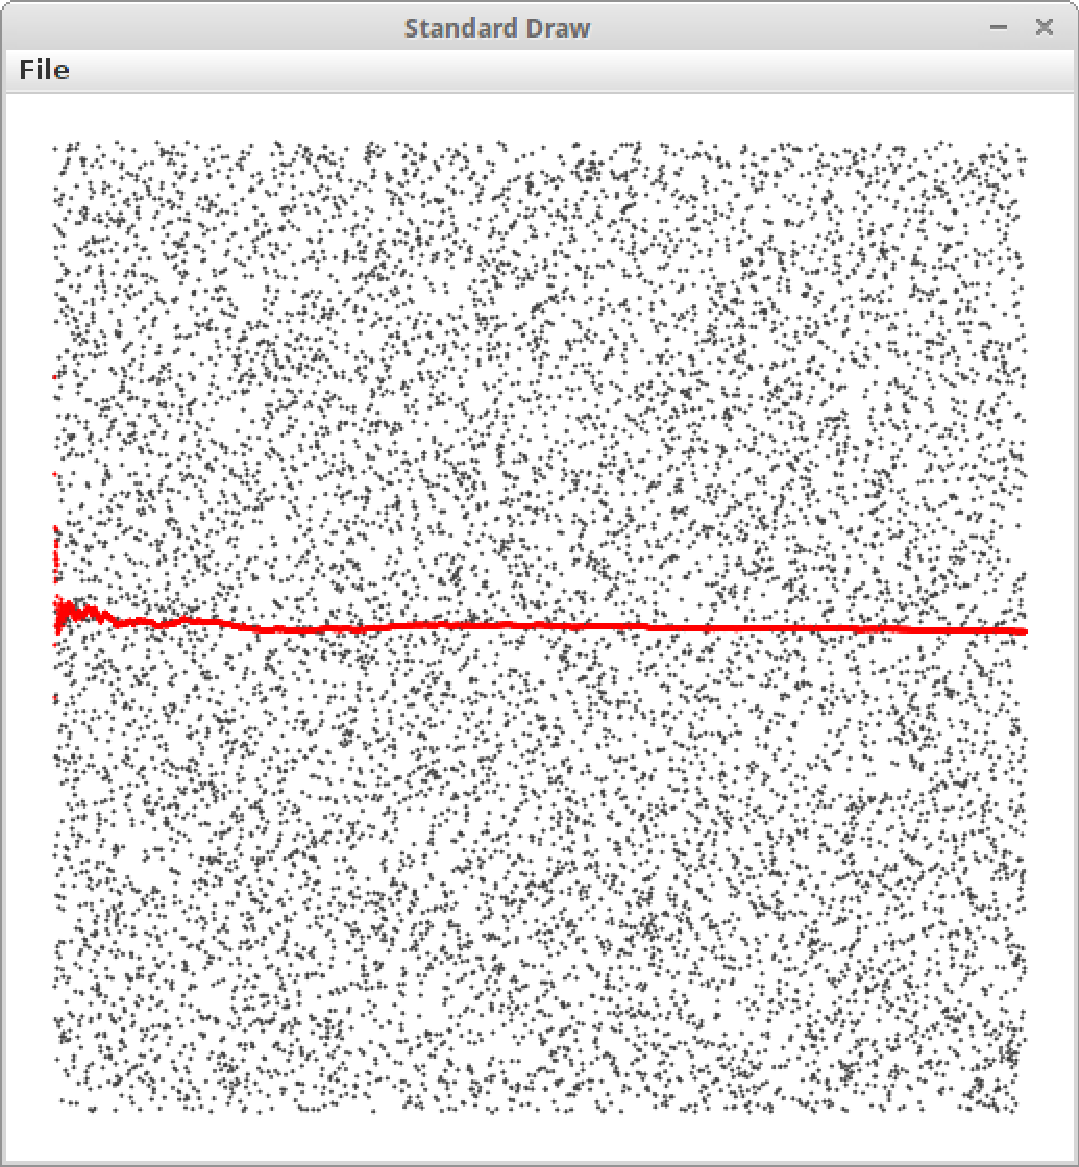
\includegraphics[scale=0.13]{./figures/visual_acc.pdf}
\end{minipage}
\end{itemize}
\end{frame}

\begin{frame}[fragile]
\begin{itemize}
\item \lstinline{VisualAccumulator} implementation
\begin{lstlisting}[language=Java]
public class VisualAccumulator {
    private double total;
    private int N;

    public VisualAccumulator(int trials, double max) {
        StdDraw.setXscale(0, trials);
        StdDraw.setYscale(0, max);
        StdDraw.setPenRadius(.005);
    }

    public void addDataValue(double val) {
        N++;
        total += val;
        StdDraw.setPenColor(StdDraw.DARK_GRAY);
        StdDraw.point(N, val);
        StdDraw.setPenColor(StdDraw.RED);
        StdDraw.point(N, mean());
    }

    public double mean() {
        return total / N;
    }

    public String toString() {
        return "Mean (" + N + " values): " + String.format("%7.5f", mean());
    }
    ...
}
\end{lstlisting}
\end{itemize}
\end{frame}

\section{Data-type Design}
\begin{frame}[fragile]
\begin{itemize}
\item encapsulation enables modular programming, allowing us to
\begin{itemize}
\item independently develop client and implementation code
\item substitute improved implementations without affecting clients
\item support programs not yet written (the API is a guide for any future client)
\end{itemize}

\item consider writing every program as though you
will need to reuse the code someday, and articulate an API for your program, providing to clients only the methods they need and no others

\item data abstraction provides a natural framework for precisely specifying both what an algorithm needs to accomplish and how a client can make use of the algorithm
\end{itemize}
\end{frame}


\begin{frame}[fragile]
\begin{itemize}
\item interface inheritance (aka subtyping) allows us to specify a relationship between otherwise unrelated classes by specifying in
an interface a set of common methods that each implementing class must contain

\item comparison interfaces (\lstinline{java.lang.Comparable} and \lstinline{java.util.Comparator})
\begin{lstlisting}[language={},mathescape]
public interface Comparable<T>

    int compareTo(T o) // compares the object with $o$ for order
\end{lstlisting}

\begin{lstlisting}[language={},mathescape]
public interface Comparator<T>

    int compare(T o1, T o2)  // compares $o_1$ and $o_2$ for order
    boolean equals(Object o) // is the comparator equal to $o$? 
\end{lstlisting}

\item \lstinline{Planet} data type
\begin{lstlisting}[language=Java]
public class Planet implements Comparable<Planet> {
    private String name;
    private int moons;

    public Planet(String name, int moons) {
        this.name = name;
        this.moons = moons;
    }
    
    public String name() { return name; }

    public int moons() { return moons; }

    public int compareTo(Planet o) { return name.compareTo(o.name); }
    
    public String toString() { return name + ", " + moons; }
}
\end{lstlisting}
\end{itemize}
\end{frame}

\begin{frame}[fragile]
\begin{itemize}
\item \lstinline{MoonComparator}
\begin{lstlisting}[language=Java]
import java.util.Comparator;

public class MoonComparator implements Comparator<Planet> {
    public int compare(Planet p1, Planet p2) { 
        return p1.moons() - p2.moons(); 
    }
    ...
}
\end{lstlisting}

\item \lstinline{Planet} test client
\begin{lstlisting}[language=Java]
import java.util.Arrays;

public class PlanetTester {
    public static void main(String[] args) {
        Planet[] planets = new Planet[8];
        planets[0] = new Planet("Mercury", 0);
        planets[1] = new Planet("Venus", 0);
        planets[2] = new Planet("Earth", 1);
        planets[3] = new Planet("Mars", 2);
        planets[4] = new Planet("Jupiter", 67);
        planets[5] = new Planet("Saturn", 62);
        planets[6] = new Planet("Uranus", 27);
        planets[7] = new Planet("Neptune", 14);
        System.out.println("Unsorted:");
        for (Planet p : planets) { System.out.println("  " + p); }
        Arrays.sort(planets);
        System.out.println("Sorted by name:");
        for (Planet p : planets) { System.out.println("  " + p); }
        Arrays.sort(planets, new MoonComparator());
        System.out.println("Sorted by # of moons:");
        for (Planet p : planets) { System.out.println("  " + p); }
    }
}
\end{lstlisting}
\end{itemize}
\end{frame}

\begin{frame}[fragile]
\begin{itemize}
\item \lstinline{Planet} test client (continued)
\begin{lstlisting}[language={}]
$ java PlanetTester 
Unsorted:
  Mercury, 0
  Venus, 0
  Earth, 1
  Mars, 2
  Jupiter, 67
  Saturn, 62
  Uranus, 27
  Neptune, 14
Sorted by name:
  Earth, 1
  Jupiter, 67
  Mars, 2
  Mercury, 0
  Neptune, 14
  Saturn, 62
  Uranus, 27
  Venus, 0
Sorted by # of moons:
  Mercury, 0
  Venus, 0
  Earth, 1
  Mars, 2
  Neptune, 14
  Uranus, 27
  Saturn, 62
  Jupiter, 67
\end{lstlisting}
\end{itemize}
\end{frame}

\begin{frame}[fragile]
\begin{itemize}
\item iteration interfaces (\lstinline{java.lang.Iterable} and \lstinline{java.util.Iterator})
\begin{lstlisting}[language={},mathescape]
public interface Iterable<T>

    Iterator<T> iterator() // an iterator over a set of elements of type T
\end{lstlisting}

\begin{lstlisting}[language={},mathescape]
public interface Iterator<E>

    boolean hasNext() // does the iteration have more elements?
    E next()          // next element in the iteration
    void remove()     // remove the last element returned
\end{lstlisting}

\item an iterable type (arrays included) can be enumerated using the enhanced for statement
\begin{lstlisting}[language=Java]
String[] dow = {"Sun", "Mon", "Tue", "Wed", "Thu", "Fri", "Sat"};
for (String s : dow) {
    StdOut.println(s);
}
\end{lstlisting}
which is (roughly) equivalent to
\begin{lstlisting}[language=Java]
String[] dow = {"Sun", "Mon", "Tue", "Wed", "Thu", "Fri", "Sat"};
Iterator iter = dow.iterator();
while (iter.hasNext()) {
    String s = iter.next();
    StdOut.println(s);
}
\end{lstlisting}
\end{itemize}
\end{frame}

\begin{frame}[fragile]
\begin{itemize}
\item \lstinline{Fibonacci} data type
\begin{lstlisting}[language=Java]
import java.util.Iterator;

public class Fibonacci implements Iterable<Long> {
    private int n;

    public Fibonacci(int n) { this.n = n; }

    public Iterator<Long> iterator() { return new FibonacciIterator(); }

    private class FibonacciIterator implements Iterator<Long> {
        private int count = 0;
        private long a = 1, b = 1;

        public boolean hasNext() { return count <= n; }

        public Long next() {
            count++;
            if (count <= 2) { return (long) 1; }
            else { 
                long t = b; b = a + b; a = t;
                return b;
            }
        }
        
        public void remove() {}
    }

    public static void main(String[] args) {
        int n = Integer.parseInt(args[0]);
        for (long i : new Fibonacci(n)) {
            StdOut.println(i);
        }
    }
}
\end{lstlisting}
\end{itemize}
\end{frame}

\begin{frame}[fragile]
\begin{itemize}
\item \lstinline{Fibonacci} data type (continued)
\begin{lstlisting}[language={}]
$ java Fibonacci 10
1
1
2
3
5
8
13
21
34
55
89
\end{lstlisting}

\item implementation inheritance (aka subclassing) enables a programmer to change behavior and add functionality without rewriting an entire class from scratch, by defining a new class (subclass or derived class) that inherits instance methods and instance variables from another class (superclass or base class)

\item every class in Java is a subclass of the \lstinline{java.lang.Object} class and therefore inherits its methods
\end{itemize}
\end{frame}

\begin{frame}[fragile]
\begin{itemize}
\item since every Java type inherits \lstinline{toString()} from \lstinline{Object}, any client can invoke \lstinline{toString()} for any object

\item wrapper types are reference types provided by Java for each of the primitive types (eg, \lstinline{Boolean} for \lstinline{boolean}, \lstinline{Integer} for \lstinline{int}, etc)

\item Java automatically converts primitive types to wrapper types (auto boxing) and wrapper types to primitive types (auto unboxing)

\item if we test equality with \lstinline{a == b} (instead of \lstinline{a.equals(b)}) where \lstinline{a} and \lstinline{b} are reference variables of the same type, we are testing whether they have the same identity, ie, the same address 

\item the ability to assign a new value to a reference variable can lead to orphaned objects
\begin{lstlisting}[language=Java]
Date a = new Date(12, 31, 2014);
Date b = new Date(1, 1, 2015);
b = a;
\end{lstlisting}

\item one of Java's most significant features is its ability to automatically manage memory (garbage collection) by keeping track of orphaned objects and returning the memory they use to a pool of free memory 
\end{itemize}
\end{frame}

\begin{frame}[fragile]
\begin{itemize}
\item an immutable data type (eg, \lstinline{Date}) has the property that the value of an object never changes once constructed

\item Java enforces immutability via the \lstinline{final} modifier

\item exceptions and errors are disruptive events that occur while a program is running

\item we have encountered exceptions thrown by Java system methods, such as   \lstinline{StackOverflowError}, \lstinline{ArithmeticException}, \lstinline{ArrayIndexOutOfBoundsException}, \lstinline{OutOfMemoryError}, and \lstinline{NullPointerException}

\item we can also raise exceptions within a program, the simplest being a \lstinline{RuntimeException} that terminates execution of the program and prints an error message
\begin{lstlisting}[language=Java]
throw new RuntimeException("Error message here.");
\end{lstlisting}

\item an assertion is a Boolean expression that we are affirming is true at that point in the program; if the expression is \lstinline{false}, the program will terminate and report an error message
\begin{lstlisting}[language=Java]
assert index >= 0;
\end{lstlisting}
or
\begin{lstlisting}[language=Java]
assert index >= 0 : "Negative index in method X";
\end{lstlisting}
\end{itemize}
\end{frame}

\end{document}
